\chapter{I processi}

\thispagestyle{empty}

Un processo è l'astrazione che indica un programma in esecuzione.
In un sistema multiprogrammato la CPU passa da un programma all'altro, eseguendo ciascuno di essi per decine o centinaia di millisecondi; ogni secondo essa può lavorare su tanti programmi diversi senza che l'utente se ne accorga.
Per indicare questo continuo alternarsi si usa l'espressione \textbf{pseudo-parallelismo}, diverso dal vero parallelismo dei sistemi multiprocessore (con più CPU quindi).

E' comunque impensabile utilizzare il 100\% della CPU, tuttavia avendo tanti processi in esecuzione ci si avvicina parecchio, vedi la figura \ref{cpu3}:

\begin{figure}[!ht]
  \centering
  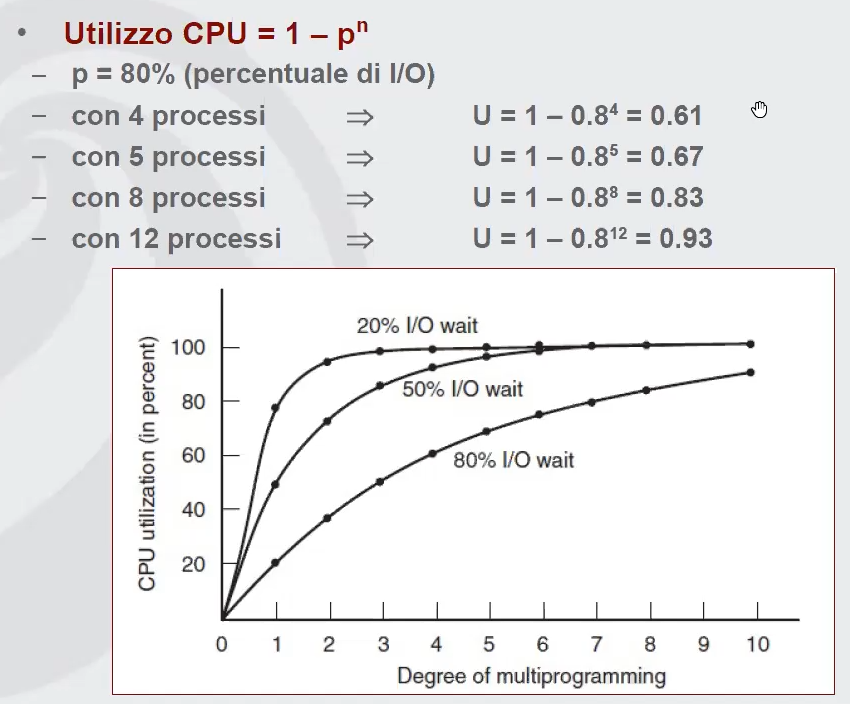
\includegraphics[width=0.6\linewidth]{assets/cpu3.png}
  \caption{stima di utilizzo della cpu}
  \label{cpu3}
\end{figure}

\section{Il modello a processi}
Ogni processo ha il suo flusso di controllo indipendente dagli altri.
Nella programmazione di processi \textbf{non} si devono fare ipotesi sulla temporizzazione. Quando un processo ha requisiti real-time critici bisogna prendere provvedimenti opportuni in modo tale che i requisiti vengano soddisfatti.

\section{La creazione dei processi}
Nei sistemi occorre avere un meccanismo per creare e distruggere i processi.
A provocare la creazione di un processo sono, principalmente, questi eventi:
\begin{enumerate}
    \item L'inizializzazione del sistema.
    \item L'esecuzione di una chiamata di sistema per la creazione di un processo, effettuata da un processo in esecuzione.
    \item Una richiesta da parte dell'utente.
    \item L'inizio di un \textit{job batch}\footnote{ Riguarda sistemi batch che si trovano in grossi mainframe, dove gli utenti possono inviare al sistema job batch anche in remoto. Quando il sistema operativo stabilisce di avere abbastanza risorse per eseguire un nuovo job crea un nuovo processo ed esegue il job successivo dalla coda.} .
\end{enumerate}

Quando un sistema operativo viene lanciato vengono creati diversi processi, alcuni che interagiscono con l'utente (\textit{foreground process}) e altri che sono eseguiti di nascosto (\textit{background process}). Questi ultimi vengono anche chiamati demoni (\textbf{daemon}).
In UNIX si usa il programma \textbf{ps} per avere informazioni sui processi attivi, in windows si premono \textit{CTRL-ALT-CANC}.
Con il comando \textit{ps} viene scattata un istantanea del sistema, per avere informazioni in tempo reale si usa il programma \textbf{top}.

In UNIX esiste una sola chiamata di sistema che crea un nuovo processo: \textbf{fork}, essa crea una copia esatta del processo chiamante. Dopo la fork i processi padre e figlio sono identici, hanno la stessa immagine di memoria (con diversi spazi di indirizzamento coinvolti, a meno di alcune eccezioni), le stesse stringhe di ambiente\dots

Normalmente il processo figlio esegue poi una \textbf{execve}, o una chiamata simile, per cambiare la sua immagine di memoria e eseguire un nuovo programma.
La ragione di questo procedimento in due passi è di permettere al figlio di manipolare i propri descrittori di file, dopo la fork e prima della execve, per realizzare la ridirezione di stdin, stdout e stderr.

\section{La terminazione dei processi}
Un processo termina al verificarsi di una di queste condizioni:
\begin{enumerate}
    \item Terminazione normale (volontaria).
    \item Terminazione con errore (volontaria).
    \item Fatal error (involontaria).
    \item Kill da un altro processo (involontaria).
\end{enumerate}

La prima si verifica con una chiamata di sistema che avvisa il sistema operativo di aver terminato i propri compiti, in UNIX è la chiamata \textbf{exit}. 
La seconda si verifica al presentarsi di un errore controllato dal programma.
La terza invece si presenta all'occorrere di un bug del codice, che causa l'esecuzione di istruzioni illegali (e.g. divisione x zero).
Per la quarta va fatto notare che il processo killer deve avere le autorizzazioni necessarie all'uccisione.

\section{Gerarchie di processi}

Il processo figlio può creare altri processi, questo porta alla formazione di una gerarchia di processi (non in windows, lì non c'è una gerarchia).
In particolare possiamo vedere come viene inizializzato UNIX: un processo speciale detto \textbf{init} è presente nell'immagine di avvio e viene lanciato. Quando inizia la sua esecuzione legge un file che dice quanti terminali ci sono, quindi si biforca creando un nuovo processo per terminale e questi processi aspettano che venga effettuato il login. Una volta effettuato il processo di login si biforca ulteriormente.. e così via. Così tutti i processi hanno come root \textit{init}.
Per verificarlo usa il comando \textbf{pstree -p}.

Un esempio di programma in C che mostra la creazione di un processo figlio:
\lstinputlisting{code/chap3.c}

\section{Gli stati dei processi}

I processi devono spesso interagire tra loro, per esempio uno potrebbe voler prendere in ingresso i dati di uscita di un altro:
\begin{verbatim}
    cat cap1 cap2 | grep tree
\end{verbatim}

In questo caso il primo processo esegue il comando \textbf{cat} che concatena i tre file, il secondo esegue \textbf{grep} che li prende in ingresso e che restituisce le righe contenenti la parola \textit{tree}.

In figura \ref{stati3} si vedono i tre stati in cui si può trovare un processo:
\begin{enumerate}
    \item Running.
    \item Ready.
    \item Blocked.
\end{enumerate}

\begin{figure}[H]
    \centering
    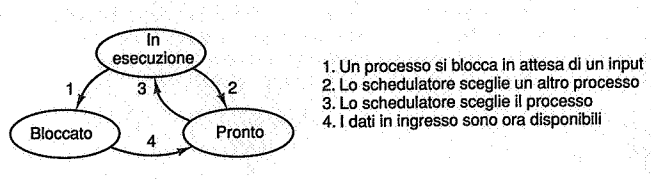
\includegraphics[width=0.6\linewidth]{assets/stati3.png}
    \caption{i possibili stati di un processo}
    \label{stati3}
  \end{figure}

  Fra questi stati sono evidenziate le quattro possibili transizioni. La seconda e la terza sono causate dallo \textbf{scheduler} (che è una parte del sistema operativo) senza che i processi se ne accorgano.
  La quarta si verifica all'occorrere di un evento esterno come l'arrivo di un dato che un processo stava attendendo.

  Fun fact: con il comando \textit{ps} in UNIX è possibile vedere i processi terminati che per qualche motivo sono ancora gestiti dallo scheduler, questi hanno indicato nel campo \textit{STAT} la dicitura \textbf{Z+}, essa sta per \textit{zombie}, ovvero processo defunto.

  Un altro modo di vedere la questione è mostrato in figura \ref{code3}, che mostra più in dettaglio i diversi tipi di situazioni nelle quali si può trovare un processo.

  \begin{figure}[H]
    \centering
    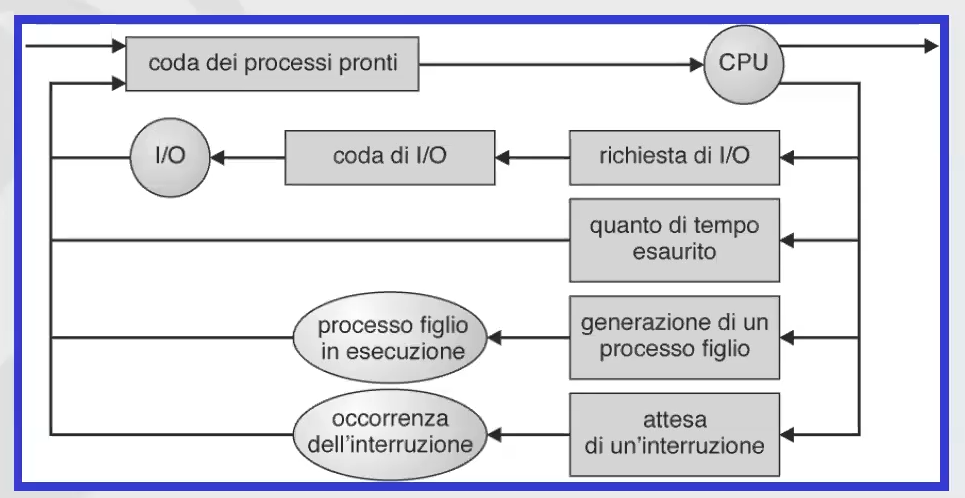
\includegraphics[width=0.7\linewidth]{assets/code3.png}
    \caption{diagramma delle code}
    \label{code3}
  \end{figure}

  \section{Implementazione}
  Per implementare il modello a processi il sistema operativo mantiene una tabella, detta \textbf{tabella dei processi}, in cui ciascun elemento referenzia un processo (gli elementi sono a volte chiamati \textbf{PCB} - Process Control Block). I PCB contengono le informazioni sullo stato del processo, il suo program counter, lo stack pointer, l'allocazione di memoria, lo stato dei suoi file aperti, le informazioni necessarie per la schedulazione e qualunque altra informazione utile per passare tra lo stato \textit{running} e gli altri stati, in maniera da far ripartire il processo al punto di interruzione, come se non si fosse mai fermato.

  Un processo UNIX spesso viene schematizzato dalle sue 4 componenti principali:
  \begin{enumerate}
    \item \textbf{u-area}: dati relativi al processo di pertinenza del sistema operativo (tabella dei file, working directory\dots).
    \item \textbf{dati}: dati globali del processo.
    \item \textbf{stack}
    \item \textbf{codice}: il codice eseguibile.
  \end{enumerate}
  
  La figura \ref{tabella3} mostra alcuni dei campi più importanti di un blocco di controllo di un sistema tipico.

  La figura \ref{azioni3} invece riassume la gestione dell'interruzione e la schedulazione.

  Infine la figura \ref{switch3} mostra un tipico \textbf{context switch}.
  
  \begin{figure}[ht]
    \centering
    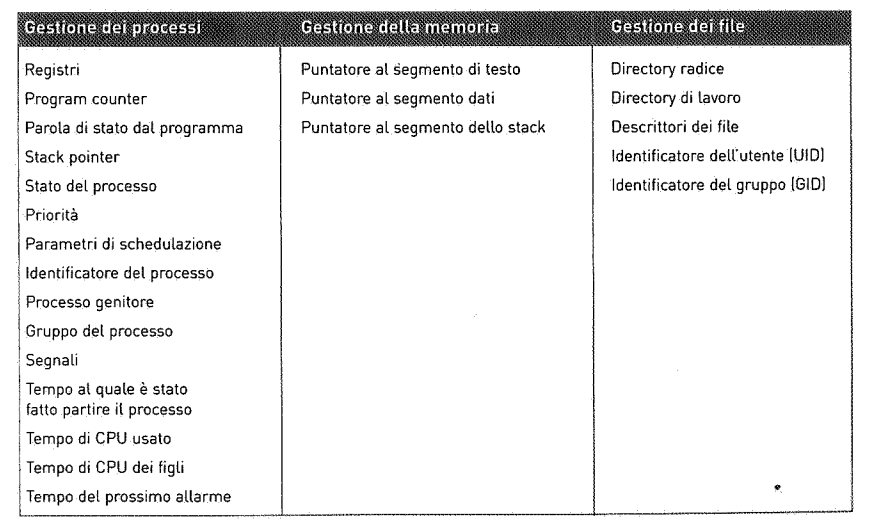
\includegraphics[width=1\linewidth]{assets/tabella3.png}
    \caption{alcuni dei campi di un elemento tipico della tabella dei processi}
    \label{tabella3}
  \end{figure}
  
  \begin{figure}[!ht]
    \centering
    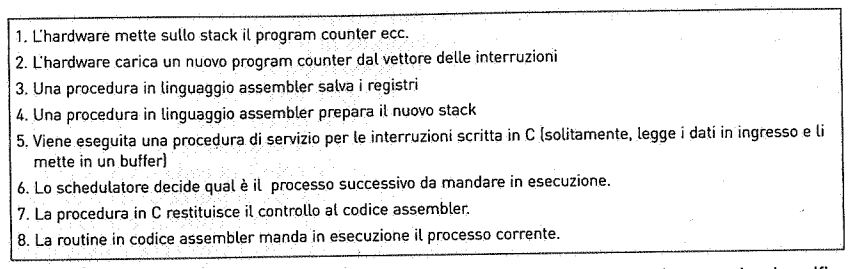
\includegraphics[width=1\linewidth]{assets/azioni3.png}
    \caption{schema delle azioni del livello più basso del sistema operativo quando si verifica un interruzione}
    \label{azioni3}
  \end{figure}

  \begin{figure}
    \centering
    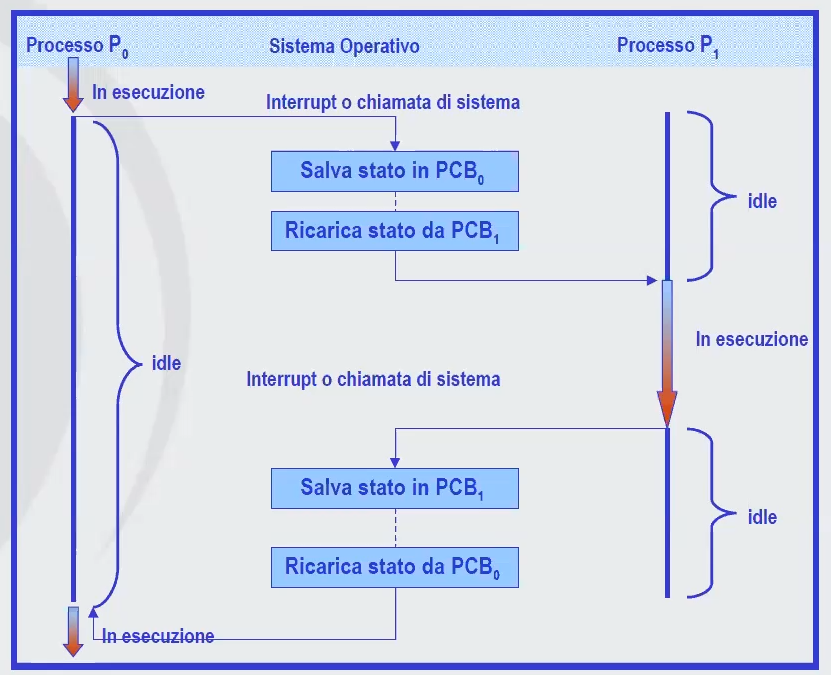
\includegraphics[width=1\linewidth]{assets/switch3.png}
    \caption{esempio di cambio di contesto}
    \label{switch3}
  \end{figure}

  \section{Miscellanea}
  \subsection{\$PATH}
  In UNIX la shell non ha bisogno del percorso dei programmi che gli vengono chiesti di eseguire, essa cerca nei percorsi indicati dalla variabile d'ambiente \textit{\$PATH}.

  \subsection{La famiglia exec}

  Esistono diversi comandi exec: \textbf{execl}, \textbf{execle}, \textbf{execlp}, \textbf{execv}, \textbf{execvp}, \textbf{execvpe}. I caratteri aggiuntivi sono: 
  \begin{itemize}
    \item \textbf{l}: passi una lista di argomenti invece di un vettore (l'ultimo elemento deve essere NULL).
    \item \textbf{e}: dopo la lista passi l'environment (variabili d'ambiente).
    \item \textbf{p}: passi, come primo parametro, la variabile di shell \textit{\$PATH}.
    \item \textbf{v}: passi con un vettore anziché una lista (ultimo elemento sempre NULL).
  \end{itemize}
L'unica effettiva chiamata di sistema è \textbf{execve}. Le altre sono usate per facilitare il programmatore.

\subsection{La funzione system}
Un'alternativa alla famiglia \textit{exec} prevede di utilizzare il comando \textbf{system}, esso accetta come parametro una stringa, che esegue in una shell come se l'utente l'avesse digitata in un terminale.